\section{Method}
\label{sec:method}

\subsection{Setup and Notation}
\label{sec:notation}

Let $A$ denote a true $K$-class categorical variable (e.g., sentiment with $K{=}3$ levels) and $A^*$ its observed, potentially misclassified version produced by an LLM annotator. The misclassification process is characterized by a $K{\times}K$ confusion matrix $C$ with entries $C_{jk} = P(A^*{=}j \mid A{=}k)$, where each column sums to one (column-stochastic: each column gives the distribution of predicted labels for a given true label). Following \citet{hernan_cole2009}, we represent this measurement process using \emph{starred-node} DAGs: the true variable $A$ is latent, and the observed $A^*$ is connected to $A$ via a dashed measurement edge.

\paragraph{Notation conventions.}
Our analysis characterizes probability limits ($N \to \infty$) under the FWL theorem~\cite{frisch1933partial}, which explains why matrix-based corrections fail for covariate topologies (Section~\ref{sec:correction}). Notation is collected in Table~\ref{tab:notation} (Appendix~\ref{app:notation_table}).

\begin{definition}[Non-differential misclassification]
\label{def:nondiff}
Misclassification of $A$ is non-differential with respect to outcome $Y$ and covariates $\mathbf{Z}$ if $P(A^*{=}j \mid A{=}k, Y, \mathbf{Z}) = P(A^*{=}j \mid A{=}k) = C_{jk}$ for all $j,k$.
\end{definition}

In batch annotation pipelines, the LLM processes each text independently without access to $Y$, making non-differentiality an architectural invariant~\cite{ziems2024can}; Y-stratified permutation tests confirm this (1/12 rejection at $\alpha{=}0.05$; Appendix~\ref{sec:nondiff_verify},~\ref{sec:y_stratified_test}). Non-differentiality may be violated when $Y$ correlates with text content, in which case our Y-stratified test provides empirical verification. Under stress testing, sign reversal occurs in 14/16 $K{\geq}3$ exposure configurations at $\eta{=}0.01$ structured departure (Appendix~\ref{sec:nondiff_stress}).

Throughout, $\tau$ denotes the causal estimand of interest, whose definition varies by topology: the confounder's coefficient, the treatment effect, the indirect effect, or the Wald ratio (Appendix~\ref{app:confounding}ff.).

We study seven canonical DAG topologies (Figure~\ref{fig:dag_taxonomy})~\cite{pearl2009, hernan2020causal}, deriving probability limits under linear structural equation models (SEMs)~\cite{carroll2006}; logistic regression robustness is verified in Appendix~\ref{sec:logistic_dgp} and~\ref{sec:fwl_nonlinear}.

\begin{figure*}[t]
\centering
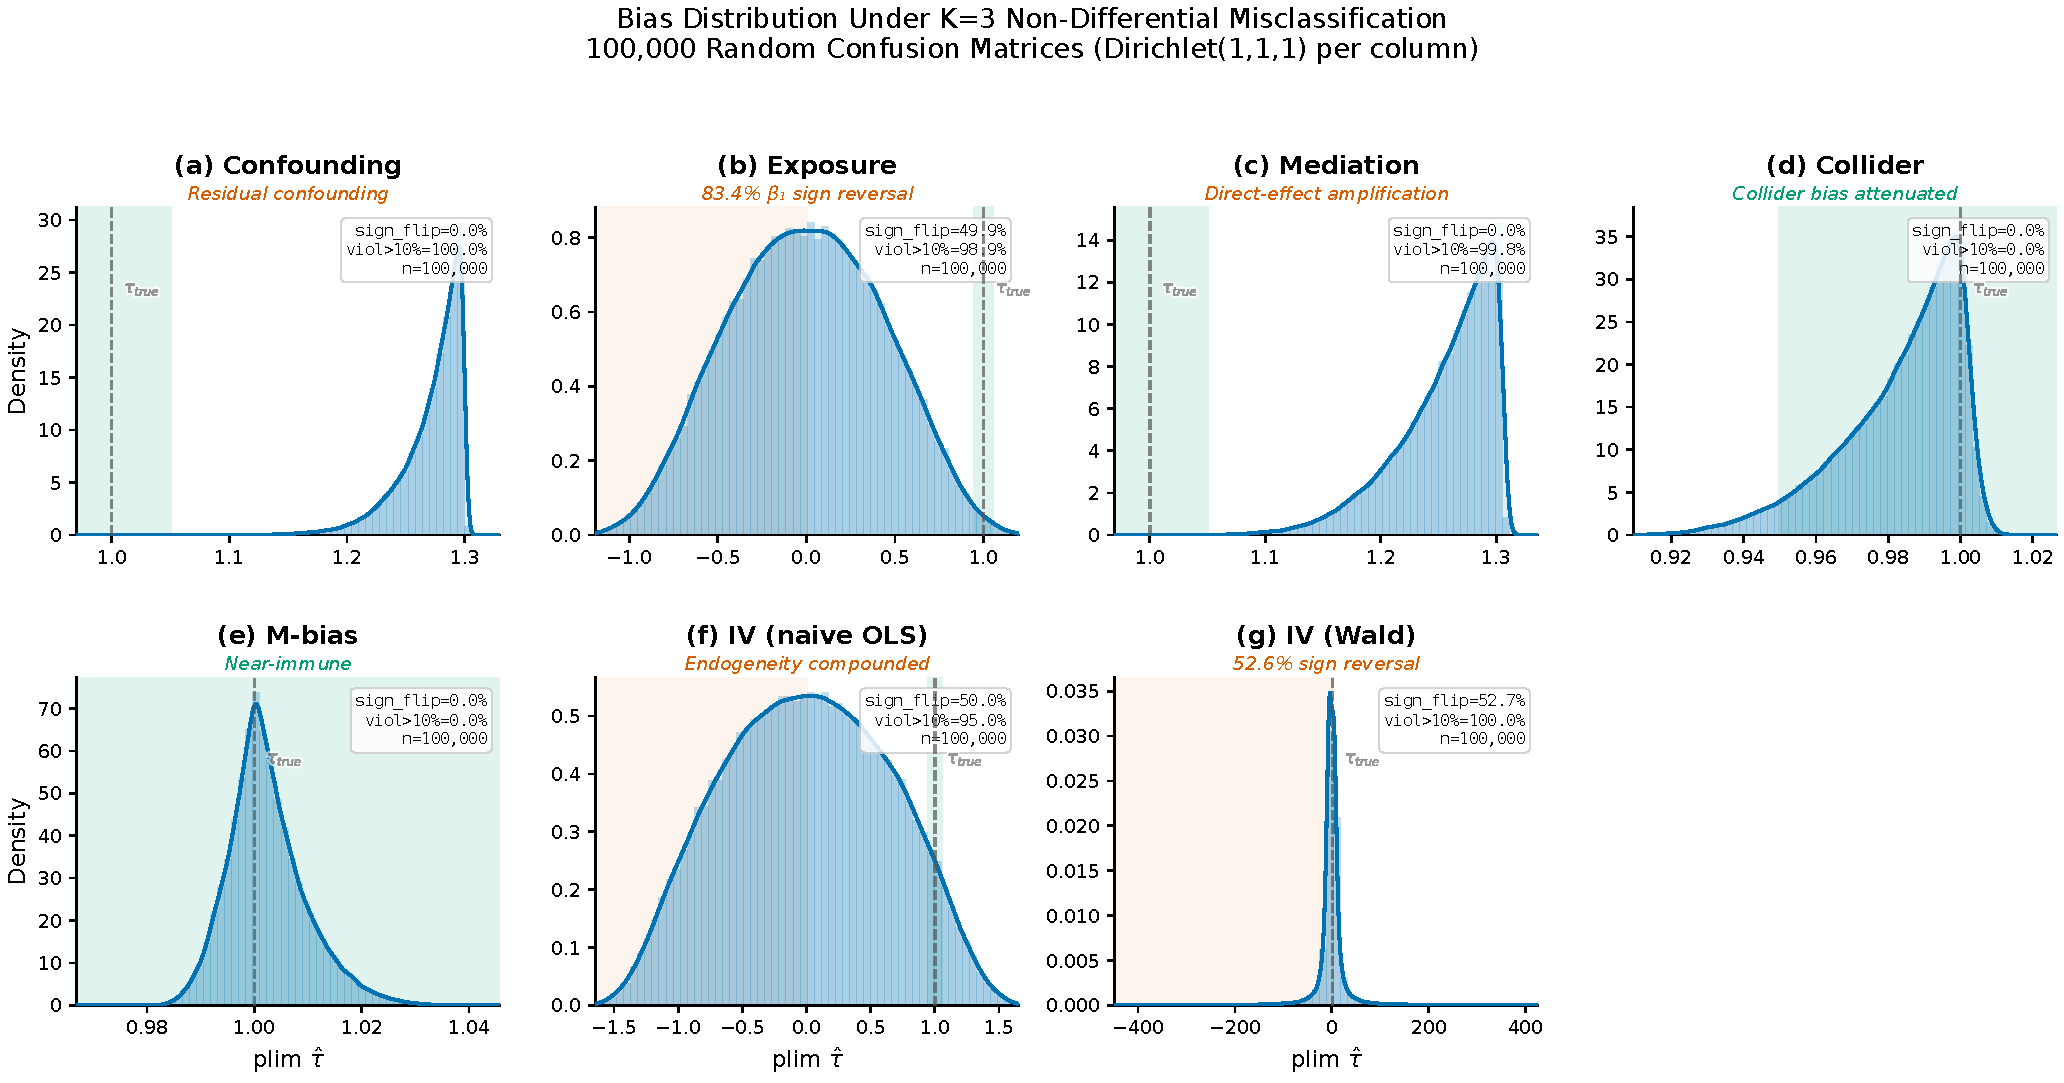
\includegraphics[width=\textwidth]{fig2_bias_distribution.pdf}
\caption{Bias distributions under 100{,}000 random $K{=}3$ confusion matrices (uniform Dirichlet; realistic-accuracy results in Section~\ref{sec:taxonomy_results}). Red = sign reversal. Exposure: 83.4\% sign reversal; IV: 52.6\%.}
\label{fig:bias_distribution}
\end{figure*}

\subsection{Multi-Class Bias Expressions}
\label{sec:bias_expressions}

For each topology, we derive the $\operatorname{plim}$\footnote{The probability limit (plim) is the value to which an estimator converges as sample size $N \to \infty$; it characterizes systematic bias separately from sampling variability.} of the naive estimator that substitutes $A^*$ for $A$. Let $\tau$ denote the target causal parameter, whose precise definition is topology-specific (e.g., the coefficient on $X$ for confounding, the category-specific $\beta_j$ for exposure, or the direct effect $\tau_{\text{direct}}$ for mediation), and $\hat{\tau}(A^*)$ the estimator using misclassified annotations.

\paragraph{Confounding ($A$ = confounder).}
When $A$ confounds the $X{\to}Y$ relationship, the ordinary least squares (OLS) estimator controlling for $A^*$ has probability limit
\begin{equation}
\label{eq:confounding}
\operatorname{plim}\;\hat{\tau}(A^*) = \bigl(\mathbb{E}[Z^{\prime}Z]\bigr)^{-1}\mathbb{E}[Z^{\prime}X]\,\boldsymbol{\beta},
\end{equation}
where $Z = [X, \text{dummies}(A^*)]$, $\boldsymbol{\beta}$ contains the true coefficients, and the target parameter $\tau$ is the coefficient on $X$. Misclassification produces residual confounding that monotonically approaches the omitted variable bias, but the sign of $\hat{\tau}$ is preserved: $\tau_{\text{sign\_flip}} = 0$ structurally.\footnote{Consistent with \citet{brenner1993}: misclassification degrades confounding control, producing amplification ($|\hat{\tau}| > |\tau|$, universal in this topology) but never sign reversal ($\operatorname{sign}(\hat{\tau}) \neq \operatorname{sign}(\tau)$).}

\paragraph{Exposure ($A$ = treatment variable).}
When $A$ is the exposure of interest, the biased coefficient for category $j$ becomes a weighted combination of true coefficients:
\begin{equation}
\label{eq:exposure}
\operatorname{plim}\;\hat{\beta}_j(A^*) = \sum_{k=1}^{K} w_{jk}\,\beta_k,
\end{equation}
where $w_{jk}$ depends on the confusion matrix $C$ and the population marginal $\pi_k = P(A{=}k)$. Unlike binary misclassification~\cite{brenner1993}, $K{\geq}3$ permits $w_{jk}$ to assign negative weight to categories with opposite-sign coefficients, producing \emph{sign reversal} (83.4\% under uniform Dirichlet prior); this is structurally impossible at $K{=}2$.

\begin{figure*}[t]
\centering
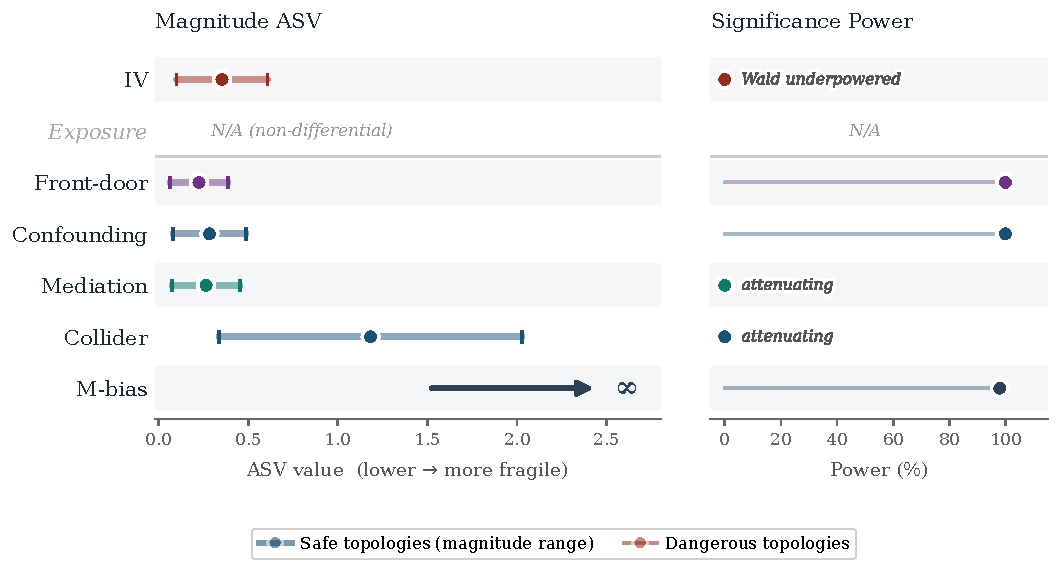
\includegraphics[width=\textwidth]{fig3_asv_ranking.pdf}
\caption{ASV vulnerability ranking across topologies. Three ASV types (magnitude, significance, sign-flip) reveal a topology-dependent spectrum from IV (maximally fragile) to M-bias (immune, ASV $= \infty$).}
\label{fig:asv_ranking}
\end{figure*}

\paragraph{Primary coefficient preservation.}
Across 23 empirical LLM configurations, the primary coefficient (the category with the largest true effect $|\beta_k|$) never reverses sign, while 61\% reverse a secondary (non-dominant) coefficient, confirmed under 100{,}000 Dirichlet matrices with diagonal ${\geq}\,0.7$ across six beta-ratio conditions (1.0 to 50.0) with 0\% primary sign-flip (Appendix~\ref{app:exposure}).

\paragraph{Mediation ($A$ = mediator).}
When $A$ mediates the $X{\to}Y$ relationship~\cite{vanderweele2015explanation}, the direct effect estimator controlling for $A^*$ has probability limit
\begin{equation}
\label{eq:mediation}
\operatorname{plim}\;\hat{\tau}_{\text{direct}}(A^*) = \tau_{\text{direct}} + \bigl(1 - \lambda(C)\bigr)\,\tau_{\text{indirect}},
\end{equation}
where $\lambda(C) \in [0,1]$ under proportional effects ($f = \lambda g$; formally stated in Theorem~\ref{thm:monotone}; Appendix~\ref{app:mediation}, Proposition~\ref{prop:lambda_bound}), with $\lambda(I) = 1$ under perfect classification. Misclassification ($\lambda < 1$) causes the residual indirect effect to be absorbed into the direct path estimate, producing upward bias in $|\hat{\tau}_{\text{direct}}|$ but preserving the sign ($\tau_{\text{sign\_flip}} = 0$).

\paragraph{Collider, M-bias, and front-door.}
Three topologies exhibit protective or immune behavior. \textbf{Collider:} conditioning on $A^*$ instead of $A$ attenuates Berkson bias by weakening the spurious path, so annotation error is protective ($\tau_{\text{sign\_flip}} = 0$). \textbf{M-bias:} in the M-shaped DAG~\cite{greenland2003}, misclassifying $A$ attenuates the non-causal path, making this topology immune ($\text{ASV} = \infty$). \textbf{Front-door:} the front-door estimator~\cite{bellemare_bloem2024} requires two stages ($X \to A$ and $A \to Y$), each attenuated by $C$; the compound effect produces moderate bias with $\tau_{\text{sign\_flip}} = 0$ (Appendix~\ref{app:frontdoor}).

\paragraph{Instrumental variable ($A$ = instrument).}
The Wald estimator~\cite{angrist_imbens1995} $\hat{\tau}_{\text{IV}} = \hat{\text{cov}}(A^*, Y) / \hat{\text{cov}}(A^*, X)$ has $C$ in the denominator. Misclassification can drive first-stage coefficients toward zero or reverse their sign; under random Dirichlet matrices, 52.6\% produce sign reversal; IV is the most fragile topology (Appendix~\ref{sec:iv_dirichlet_subspace}).

\paragraph{Structural sign-flip guarantee.}
\begin{proposition}[Sign preservation: analytic results]
\label{prop:signflip}
Under non-differential misclassification with $C_{kk} > 0$ for all $k$:
\emph{(a)}~Confounding preserves sign when $\operatorname{sign}(\tau) = \operatorname{sign}(\tau {+} B_{\mathrm{OV}})$, where $B_{\mathrm{OV}} {=} \operatorname{Cov}(g(A),f(A))/\operatorname{Var}(T)$ is the omitted-variable bias (Cauchy--Schwarz; Appendix~\ref{app:confounding}).
\emph{(b)}~Collider preserves sign when $|\tau| > \sqrt{\operatorname{Var}(g)\operatorname{Var}(h)}/\mathbb{E}[\operatorname{Var}(T{\mid}A)]$ (Berkson attenuation; Appendix~\ref{app:collider}); empirically verified across 100{,}000 matrices with zero violations.
\emph{(c)}~Exposure can produce sign reversal for $K {\geq} 3$, even with $C_{kk} {>} 0.5$ (counterexample in Appendix~\ref{app:exposure}).
\end{proposition}

Sign preservation for non-exposure topologies holds under topology-specific conditions (Table~\ref{tab:sign_conditions}, Appendix~\ref{app:conditions}), verified across 100{,}000 random matrices with zero violations; analytic proofs for general $K$ remain open.

\subsection{Annotation Sensitivity Values}
\label{sec:asv}

We adapt the sensitivity analysis paradigm (E-values~\cite{vanderweele_ding2017}, partial-$R^2$ bounds~\cite{cinelli2020making}, coefficient stability~\cite{oster2019}) to $K{\times}K$ annotation error and define Annotation Sensitivity Values (ASVs): we prove $\varepsilon$-approximate monotonicity along $C(\delta)$ (Theorem~\ref{thm:monotone}), which reduces $K^2$ dimensions to a scalar; define three ASV diagnostics for topology-dependent failure modes; and combine ASVs with FWL invariance to route corrections.

\paragraph{Parameterization.}
We set $C(\delta) = (1{-}\delta)I + \delta C_0$, where $C_0$ is a reference confusion matrix and $\delta \in [0,1]$ controls severity ($\delta{=}0$: perfect; $\delta{=}1$: matches $C_0$). This linear path is one of many in the column-stochastic polytope from $I$ to $C_0$; ASV thresholds are path-dependent, but our bootstrap procedure (Section~\ref{sec:asv_results}) captures estimation uncertainty along the empirical path. We recommend bootstrapping $C_0$ and reporting ASV confidence intervals (Appendix~\ref{sec:bootstrap_asv}).
\paragraph{Three ASV types.}
We define three complementary measures: (1)~\textbf{Magnitude ASV} $\delta^*_{\text{mag}} = \min\{\delta : |\operatorname{plim}\;\hat{\tau}(C(\delta)) - \tau| > \epsilon\}$, analogous to E-values; (2)~\textbf{Significance ASV} $\delta^*_{\text{sig}} = \min\{\delta : |\operatorname{plim}\;\hat{\tau}(C(\delta))| < z_{\alpha/2} \cdot SE(N)\}$, relevant for attenuating topologies; (3)~\textbf{Sign-flip ASV} $\delta^*_{\text{sf}} = \min\{\delta : \operatorname{sign}(\hat{\tau}) \neq \operatorname{sign}(\tau)\}$, for exposure and IV only. The significance ASV depends on $N$ through $SE(N)$, exhibiting a sharp phase transition at a critical $N^*$ below which all rejections are blocked.

\begin{theorem}[Envelope monotonicity, $K{=}2$]
\label{thm:monotone}
For $K{=}2$ confounding and mediation topologies with proportional effects ($f = \lambda g$ for some scalar $\lambda$) under $C(\delta) = (1{-}\delta)I + \delta C_0$ with $(C_0)_{jj} \geq \tfrac{1}{2}$, $|B(C(\delta))|$ is monotonically non-decreasing in $\delta \in [0,1]$.
\end{theorem}

The proof (Appendix~\ref{app:monotonicity_proof},~\ref{par:med_monotone}) exploits perspective function convexity. All 23 empirical configurations preserve sign; 97.3\% do so under non-proportional effects (Appendix~\ref{sec:proportional_effects}).

\begin{theorem}[$K{=}3$ symmetric monotonicity]
\label{thm:k3_symmetric}
For $K{=}3$ with symmetric confusion matrix $C_{jk} = c$ for $j \neq k$ and $C_{kk} = 1{-}2c$, $c \in (0, 1/3)$, and proportional effects ($f{=}\lambda g$), envelope monotonicity holds exactly: $|B(C(\delta))|$ is strictly monotone in $\delta$ for confounding, mediation, and collider topologies whenever $\mathrm{Var}(g) > 0$.
\end{theorem}

Theorem~\ref{thm:k3_symmetric} anchors exact monotonicity at $K{=}3$; for general asymmetric matrices ($d_{\mathrm{rel}}{=}0.33$; Remark~\ref{rem:symmetry}), Conjecture~\ref{conj:monotone} provides $\varepsilon < 0.017$ coverage. The proof exploits the reduction $s = c\delta$ (Appendix~\ref{app:k3_symmetric_proof}).

\paragraph{From proofs to numerical evidence.}
Exact monotonicity (Theorems~\ref{thm:monotone}--\ref{thm:k3_symmetric}) does not extend to general $K{\geq}3$ column-stochastic structures; we state a conjecture supported by numerical evidence:

\begin{conjecture}[$\varepsilon$-approximate envelope monotonicity]
\label{conj:monotone}
For general $K{\geq}3$ non-IV topologies under $C(\delta) = (1{-}\delta)I + \delta C_0$, $|B(C(\delta))|$ is $\varepsilon$-approximately monotonic with $\varepsilon < 0.02$ for $|\beta| \leq 1$, scaling with effect magnitude (Table~\ref{tab:conjecture_verify},~\ref{tab:dgp_sensitivity}; Appendix~\ref{sec:conjecture_verify}). The safe/fragile partition (five sign-preserving topologies versus exposure and IV) is robust across all tested parameterizations.
\end{conjecture}

Numerical support spans 100{,}000 Dirichlet matrices and 545{,}945 adversarial curves (Appendix~\ref{app:adversarial_monotonicity}).

\begin{remark}[ASV and E-values as complementary tools]
\label{rem:evalue}
ASV and E-values~\cite{vanderweele_ding2017} address orthogonal sources (annotation error vs.\ unmeasured confounding; Appendix~\ref{sec:sensitivity_comparison}) and are most valuable jointly.
\end{remark}

Under alternating-sign effects ($\boldsymbol{\beta}{=}[0,\,1.0,\,-0.5]$), magnitude ASV ranges from 0.09 (exposure) to $\infty$ (M-bias), a $4{\times}$ difference determined by topology (Table~\ref{tab:asv_stability}). Sign-flip ASV $< 1$ flags sign-reversal-prone pairs; magnitude ASV $< \delta_{\text{observed}}$ indicates bias exceeds tolerance (Algorithm~\ref{alg:correction}); the safe/fragile partition is stable across parameterizations ($\varepsilon < 0.02$; Appendix~\ref{sec:asv_stability}).
